\NeedsTeXFormat{LaTeX2e}
\documentclass[11pt]{article}
%Absaetze nicht einruecken:
\usepackage{parskip}
\usepackage[utf8]{inputenc}
\usepackage[T1]{fontenc}
\usepackage{ae}
\usepackage[intlimits, sumlimits, namelimits]{amsmath}
\usepackage{bbm}
%Neue Macros fuer Mathe:
%in parentheses - gleich mit richtiger Groesse
\newcommand{\inp}[1]{\ensuremath{\left(#1\right)}}
\newcommand{\sqr}{\ensuremath{^{2}}}
\newcommand{\cube}{\ensuremath{^{3}}}
%Mengensymbole mit doppelten senkrechten Strichen:
\newcommand{\set}[1]{\ensuremath{\mathbbm{#1}}}
%definiert eine Norm, also zwei senkrechte Striche auf jeder Seite:
\newcommand{\norm}[1]{\ensuremath{\left|#1\right|}}
%Spaltenvektor - dreidimensional:
\newcommand{\svec}[3]{\ensuremath{\inp{\hspace{-.8ex}\begin{array}{r}#1\\#2\\#3\end{array}\hspace{-.4ex}}}}
\newcommand{\entspr}{\ensuremath{\,\,\hat{=}\,\,}}%
\newcommand{\dx}[1][x]{\ensuremath{\textnormal d #1}}

% For stupid thinkos:
\newcommand{\cross}{\times}

% Tabellen:
\usepackage{array}
\setlength{\extrarowheight}{.2mm}
%Links im Text:
\usepackage{hyperref}
\usepackage{graphics,graphicx,fancyvrb}
%Raender einstellen
%\usepackage[a4paper, margin=15mm, top=30mm]{geometry}
\usepackage[a4paper]{geometry}
%Kopf - und Fusszeilen
\usepackage{lastpage}
\usepackage{fancyhdr}
	\lhead{Moritz Lenz}
	\chead{\bfseries{-- \thepage\ --}}
	\rhead{\thetitle}
	\lfoot{}
	\rfoot{}
	\cfoot{}
	\pagestyle{fancy}
\pagestyle{empty}

\sffamily

%Kopfzeile

\author{Moritz Lenz}
\title{Adaption between chiral and spin up/down bases}
\begin{document}
\maketitle

The chiral spin bases are very natural for the analytical calculation, because the
base vectors are also eigenstates to the Hamiltonian.

However for the numerical simulation they are not suited, because they are
dependent on the direction (in real space) in which the wave travels. This
that's not known before the simulation runs, and because there can be several
waves with different directions in one place, it is not possible to calculate
the self-energy of the leads in these bases.

\begin{figure}
    \begin{center}
    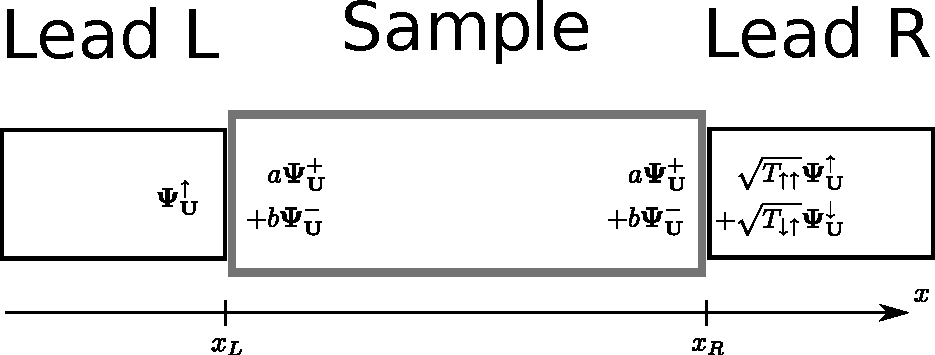
\includegraphics[width=0.8\textwidth]{adapting-pic.pdf}
    \end{center}
    \caption{Injecting one spin-up charge carrier into the system}
\end{figure}

% Since there is no dissipation in our model, and we assume that the mere
% process of injecting an electron doesn't change its spin, we can project
% the $|\uparrow>$ and $|\downarrow>$ states separately onto the wave
% function in the sample:

Since we assume that our leads are perfect semi-infinite wires, we can assume
that the wave functions are plain waves

\begin{align*}
    \mathbf{\Psi^\uparrow}   &=  e^{i p_x x} e^{i p_z z} |\uparrow> \\
    \mathbf{\Psi^\downarrow} &=  e^{i p_x x} e^{i p_z z} |\downarrow> \\
\end{align*}

and that the wave functions are continuous at the interface:

\begin{align*}
    \mathbf{\Psi^\uparrow}(x=x_L) &=
        a \mathbf{\Psi^+_U}(x=x_L) + b  \mathbf{\Psi^-_U}(x=x_L)\\
    \mathbf{\Psi^\downarrow}(x=x_L) &=
        c \mathbf{\Psi^+_U}(x=x_L) + d  \mathbf{\Psi^-_U}(x=x_L)
\end{align*}

Where $x_L$ is the location where the left lead is connected to the sample, the
interface is at $x = 0$ and the right lead is connected at $x = x_R$.
Each of these equations has two components, which allows us to determine
$a, b, c$ and $d$ unambiguously.

With $\mathbf{\Psi^\pm_U}$ we mean the wave function normalized to 1 at the
left hand side of the interface, so for example
$|\mathbf{\Psi^\pm_U}(x=x_L)|=1$. 

We can then look at the connection to the right lead, and obtain a matrix
element of the transmission matrix in the $\uparrow, \downarrow$ bases:

\begin{align*}
    T_{\uparrow\uparrow} = \left| \left( 
        a \mathbf{\Psi^+_U}(x=x_R) + b  \mathbf{\Psi^-_U}(x=x_R)
    \right)^\dagger \cdot \mathbf{\psi^\uparrow}(x=x_R) \right|^2
\end{align*}

\end{document}

% vim: ts=4 sw=4 expandtab spell spelllang=en_us
